 \documentclass[t]{beamer}
%\documentclass[c]{beamer}
\listfiles

\mode<presentation>
{
%  \usetheme[english,titlepage0]{KIT}
  \usetheme[titlepage0]{KIT}
% \usetheme[usefoot]{KIT}
% \usetheme[deutsch]{KIT}

%%  \usefonttheme{structurebold}

  \setbeamercovered{transparent}

  %\setbeamertemplate{enumerate items}[circle]
  \setbeamertemplate{enumerate items}[ball]
}

\usepackage{babel}
%\date{10.05.2010}
%\DateText

%\newlength{\Ku}
%\setlength{\Ku}{1.43375pt}

\usepackage[latin1]{inputenc}
\usepackage[TS1,T1]{fontenc}
\usepackage{array}
\usepackage{multicol}
\usepackage{lipsum}

%\usenavigationsymbols
%\usenavigationsymbols[sfHhdb]
%\usenavigationsymbols[sfhHb]

\title{Example for a Title}
%\subtitle{Example for a Subtitle}

\author{KIT}

\institute[\raisebox{-3.5mm}{
\includegraphics[height=\KITlogoht]{Bilder/Zlogo}}]
  {INSTITUTS- FAKULT�TS-, ABTEILUNGSNAME}
\logo{
\includegraphics[width=\KITlogowd]{Bilder/Zlogo}}

\TitleImage[height=\titleimageht]{Bilder/bildwand.jpg}

\newcommand{\itemsiii}{
  \item Uter res comprovincialis placitum opus alo Liceo, ploro an at lenocinium.
        Iuste Immanitas dux sus conclamo an Diuturnus
  \item Fatigo, almus ut erro cupido res famulatus Adstringo
  \item Stupendum commemoro Annuo ars quies Polliceor
}
\newcommand{\itemsi}{
  \item Ne necne Ne ymo iam Vota, Rutilus dux scelus internuntius.
}


\newcommand{\parxmpl}{
  Uter res comprovincialis placitum opus alo Liceo, ploro an at lenocinium.
  Iuste Immanitas dux sus conclamo an Diuturnus
  Fatigo, almus ut erro cupido res famulatus Adstringo
  Stupendum commemoro Annuo ars quies Polliceor
}
\newcommand{\Parxmpl}{
  Iuste Immanitas dux sus conclamo an Diuturnus
  Fatigo, almus ut erro cupido res famulatus Adstringo
}

\begin{document}

\begin{frame}
  \maketitle
\end{frame}

\begin{frame}
  \frametitle{Image and Text 1}

  \begin{columns}[T]
    \column{57mm}
    \begin{itemize}\small
    \itemsi
    \itemsiii
    \end{itemize}
    \column{50mm}
    \hspace*{-6mm}\hfill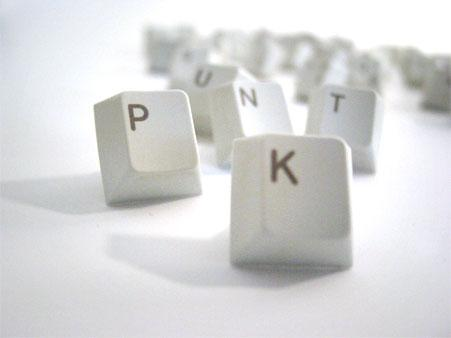
\includegraphics[width=54mm]{Bilder/tasten.jpg}
  \end{columns}
\end{frame}

\begin{frame}
  \frametitle{Image and Text 2}
  \framesubtitle{Starting with a Picture}

  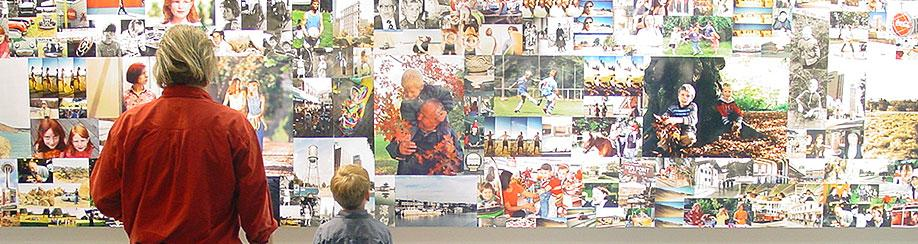
\includegraphics[width=\textwidth]{Bilder/bildwand.jpg}

  \begin{itemize}\small
  \itemsi
  \itemsiii
  \end{itemize}
  \vfill
  \mbox{}
\end{frame}
\end{document}
